\begin{center}
\graphicspath{{/root/R-project/IFishSnapperWPP573/Images/}}
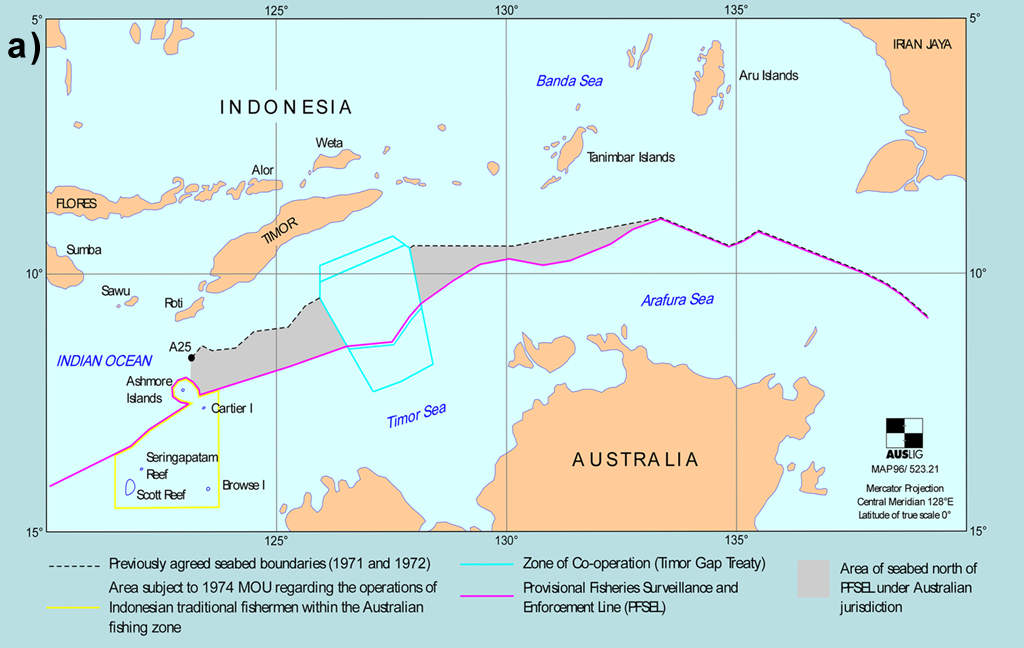
\includegraphics[scale=0.4]{JPDA-Map.png}
\end{center}

\begin{wrapfigure}{r}{8cm}
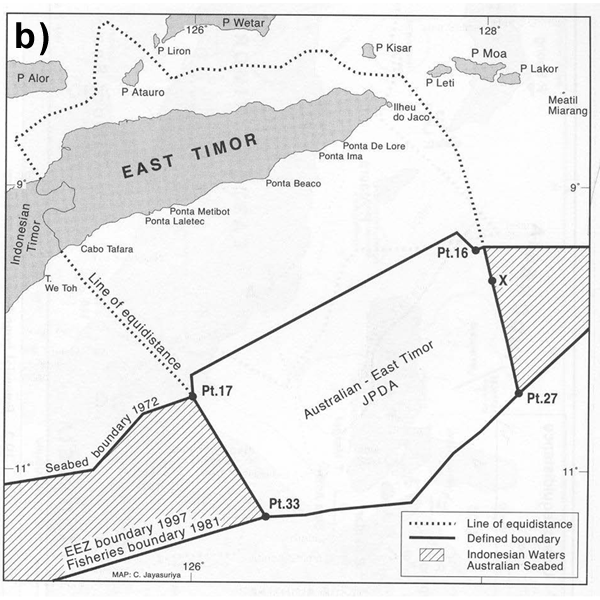
\includegraphics[width=1\linewidth]{/root/R-project/IFishSnapperWPP573/Images/JPDA-Map-bw.png}
\end{wrapfigure}

Figure 8. Timor Sea fishing grounds with current boundaries between Indonesia, East Timor and Australia.

a) The dotted line is the Australia - Indonesia Seabed Boundary. The pink line (PFSEL) is the Australia - Indonesia Fisheries Boundary. Indonesian vessels are allowed to fish in the grey area between the pink line and the dotted line, but not below the PFSEL. The light blue line is the boundary of the East Timor - Australia Zone of Cooperation which covers East Timorese fishing grounds where Indonesian fishing vessels are not allowed to fish. Australia does not enforce fisheries regulations here.

b) The shaded area between the Seabed Boundary and the Fisheries Boundary is Australian seabed, where fishers from Indonesia are allowed to fish. The Australian - East Timor zone of cooperation or �Joint Petroleum Development Area� (JPDA) is not open to fishers from Indonesia. East Timor is responsible for fishery surveillance within the JPDA.

Source: Australian Surveying \& Land Information Group (AUSLIG) Commonwealth Department of Industry Science and Resources. MAP 96/523.21.1.

\clearpage
\newpage

The presented Spot trace data from the Timor Sea drop line fisheries illustrate a classic "fishing the line" phenomenon. The vessels mainly fish right at the Indonesia - Australia border, on the edge of better managed fishing grounds on the Australian side, where fish densities are higher and individual fish are larger. Additional fishing takes please near Rote Island and a few other locations on the boundary of the Savu and Timor Seas. Several drop line fishers were observed to operate illegally in Australian waters and some of these have been arrested by Australian patrol boats in 2015.

Some drop line and especially long line vessels have also been observed to illegally fish in Timor Leste waters. There is apparently little or no enforcement of fisheries regulations in Timor Leste waters and especially the Joint Petroleum Development Area or JPDA (an area in Timor Leste waters where a resource sharing agreement for seabed resources is in place with Australia) is frequently targeted illegally by Indonesian vessels.

\begin{center}
\graphicspath{{/root/R-project/IFishSnapperWPP573/Images/}}
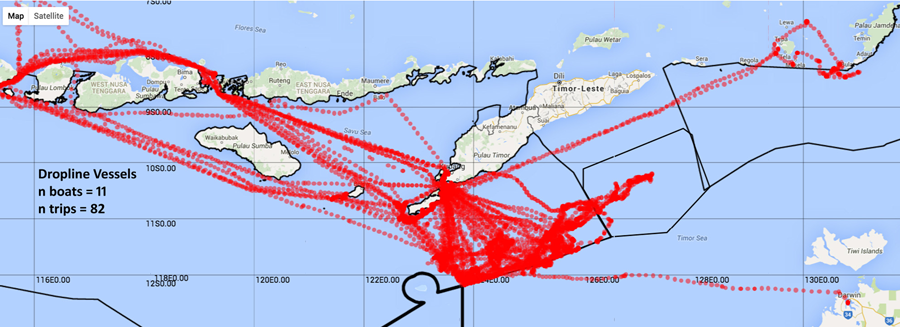
\includegraphics[scale=0.5]{DroplineVesselsTimorSea.png}

Figure 9. Map with aggregated Spot Trace data from deep drop line vessels. Dots in a line represent the tracks of a travelling fishing vessel whereas dots in a cluster represent fishing activity. The dotted line to Darwin shows an Indonesian fishing vessels arrested by Australian navy.
\end{center}

\begin{center}
\graphicspath{{/root/R-project/IFishSnapperWPP573/Images/}}
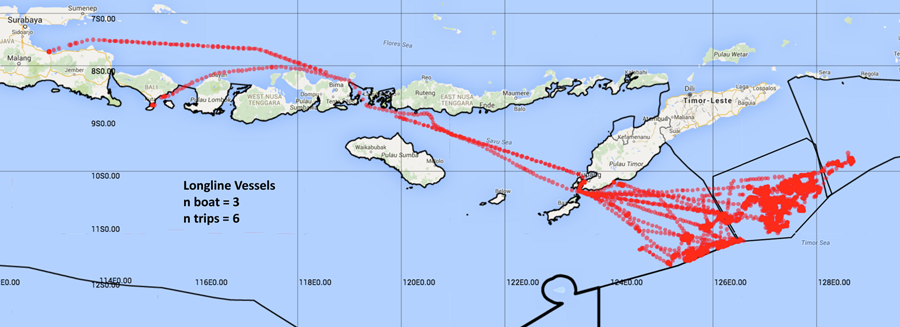
\includegraphics[scale=0.5]{LonglineVesselsTimorSea.png}

Figure 10.  Map with aggregated Spot Trace data from bottom long line vessels. Dots in a line represent the tracks of a travelling fishing vessel whereas dots in a cluster represent fishing activity.
\end{center}




